\documentclass[12pt]{article}
\usepackage[portuguese]{babel}
\usepackage[utf8]{inputenc}
\usepackage{indentfirst}
\usepackage{graphicx}
\usepackage{verbatim}
\usepackage{natbib}
\usepackage{float}
\usepackage{hyperref}
\usepackage{amsmath}
\usepackage{listings}  
\usepackage{mathtools}
\usepackage{filecontents}
\usepackage{graphicx}
\usepackage{caption}
\usepackage{algorithm}
\usepackage{algpseudocode}
\usepackage{subcaption}
\graphicspath{ {images/} }
\usepackage{parskip}
\usepackage{fancyhdr}
\usepackage{vmargin}
\usepackage{wrapfig}
\newcommand\tab[1][1cm]{\hspace*{#1}}
\setmarginsrb{2.75 cm}{2.5 cm}{2.75 cm}{2.5 cm}{1 cm}{1.5 cm}{1 cm}{1.5 cm}

\title{Corrida de Reis}													% Title
\author{Afonso Jorge Ramos}											% Author
\date{12th October 2017}												% Date

\makeatletter
\let\thetitle\@title
\let\theauthor\@author
\let\thedate\@date
\makeatother

\pagestyle{fancy}
\fancyhf{}
\rhead{Programação em Lógica}
\lhead{\thetitle}
\cfoot{\thepage}

\DeclareCaptionFormat{algor}{%
  \hrulefill\par\offinterlineskip\vskip1pt%
    \textbf{#1#2}#3\offinterlineskip\hrulefill}
\DeclareCaptionStyle{algori}{singlelinecheck=off,format=algor,labelsep=space}
\captionsetup[algorithm]{style=algori}

\begin{document}

%%%%%%%%%%%%%%%%%%%%%%%%%%%%%%%%%%%%%%%%%%%%%%%%%%%%%%%%%%%%%%%%%%%%%%%%%%%%%%%%%%%%%%%%%

\begin{titlepage}
	\centering
    
	
    \textsc{\LARGE Faculdade de Engenharia \\ da Universidade do Porto}\\[2.0 cm]	% University Name

\includegraphics[scale = 0.15]{feup-logo.png}\\[1.5 cm]							% University Logo
	\textsc{\Large Relatório Intercalar}\\[0.8 cm]							% Course Code
	\textsc{\large Programação em Lógica \\[0.8 cm] Mestrado Integrado em Engenharia Informática e
Computação}\\[0.5 cm]													% Course Name
	\rule{\linewidth}{0.2 mm} \\[0.4 cm]
	{ \huge \bfseries \thetitle}\\
	\rule{\linewidth}{0.2 mm} \\[1.5 cm]
	
	\begin{minipage}{0.4\textwidth}
		\begin{flushleft} \large
			\emph{Autores:}\\
			\theauthor \\ João Dias Conde Azevedo
			\end{flushleft}
			\end{minipage}~
			\begin{minipage}{0.4\textwidth}
			\begin{flushright} \large
			\emph{} \\
			up201506239@fe.up.pt	\\  up201503256@fe.up.pt
		\end{flushright}
	\end{minipage}\\[2 cm]
	
	{\large \thedate}\\[3 cm]
 
	\vfill
	
\end{titlepage}

%%%%%%%%%%%%%%%%%%%%%%%%%%%%%%%%%%%%%%%%%%%%%%%%%%%%%%%%%%%%%%%%%%%%%%%%%%%%%%%%%%%%%%%%%

\tableofcontents
\pagebreak

%%%%%%%%%%%%%%%%%%%%%%%%%%%%%%%%%%%%%%%%%%%%%%%%%%%%%%%%%%%%%%%%%%%%%%%%%%%%%%%%%%%%%%%%%

%Todas as figuras devem ser referidas no texto. %\ref{fig:codigoFigura}
%
%%Exemplo de código para inserção de figuras
%%\begin{figure}[h!]
%%\begin{center}
%%escolher entre uma das seguintes três linhas:
%%\includegraphics[height=20cm,width=15cm]{path relativo da imagem}
%%\includegraphics[scale=0.5]{path relativo da imagem}
%%\includegraphics{path relativo da imagem}
%%\caption{legenda da figura}
%%\label{fig:codigoFigura}
%%\end{center}
%%\end{figure}
%
%
%\textit{Para escrever em itálico}
%\textbf{Para escrever em negrito}
%Para escrever em letra normal
%``Para escrever texto entre aspas''
%
%Para fazer parágrafo, deixar uma linha em branco.
%
%Como fazer bullet points:
%\begin{itemize}
	%\item Item1
	%\item Item2
%\end{itemize}
%
%Como enumerar itens:
%\begin{enumerate}
	%\item Item 1
	%\item Item 2
%\end{enumerate}
%
%\begin{quote}``Isto é uma citação''\end{quote}


%%%%%%%%%%%%%%%%%%%%%%%%%%

\section{Corrida de Reis}

Esta variante do xadrez tradicional, Corrida de Reis, inventada por Vernon R. Parton em 1961, tem por objectivo levar o próprio rei até à última linha antes do adversário. 

Vernon Rylands Parton foi um entusiasta de xadrez e um inventor prolífico de variantes para o mesmo, sendo o Xadrez de Alice a variante por ele criada mais conhecida. Muitas das variantes por ele inventadas possuíam inspiração de personagens fictícias e histórias dos trabalhos de Lewis Caroll. Parton, tal como Lewis Caroll, dedicou grande parte da sua vida académica à matemática, mas possuia interesses vários na ciência e era um forte apoiante de Esperanto.

\begin{wrapfigure}{R}{0.4\textwidth}
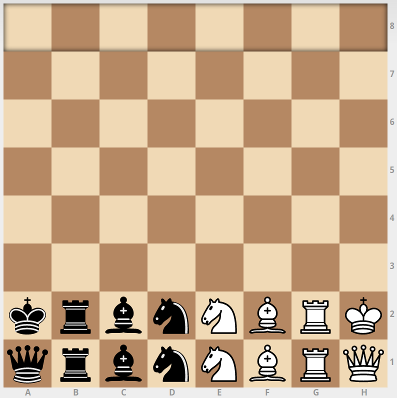
\includegraphics[width=0.9\linewidth]{racing.png} 
\caption{Tabuleiro base.}
\label{fig:subim1}
\end{wrapfigure}
Já face ao jogo em causa, Corrida de Reis, cada jogador começa o jogo com todas as peças normalmente usadas no xadrex exceto os peões, ou seja, começa com 1 rei, 1 rainha, 2 torres, 2 bispos e 2 cavalos. Todas as peças (brancas e pretas) são colocadas nas primeiras duas linhas do tabuleiro e ambos os jogadores veêm o jogo da mesma prespectiva. Assim, o tabuleiro inicial tem o aspeto especificado na figura1.

Como já referido, o objectivo é ser o primeiro a levar o próprio rei até à última linha (linha 8), usando as regras do Xadrez tradicional para mover e capturar as peças. 

Contudo, impoem-se restrições adicionais, listadas abaixo:
\begin{description}
  \item[$\bullet$] Não é permitido atacar o rei adversário, isto é, não se podem efetuar jogadas que colquem o rei adversário em cheque;
  \item[$\bullet$] Um rei não pode mover-se para uma casa coberta por uma peça adversária.
\end{description}
Visto que para alcançar a vitória, um jogador deve mover o seu rei para a última linha, o jogador correspondente às peças brancas possuiría uma vantagem clara, por começar primeiro. Assim, quando é o rei branco que chega primeiro à última linha, o jogador preto tem uma ronda extra para que, caso consiga colocar o seu rei na última linha nessa jogada, declara-se um empate. Desta forma compensa-se a vantagem que as brancas têm por jogarem primeiro.


%%%%%%%%%%%%%%%%%%%%%%%%%%
\section{Representação do Estado do Jogo}

O estado de jogo é guardado no tabuleiro, representado por uma lista de listas.
O tabuleiro é de 8x8 e, por isso, a primeira lista conterá outras 8, cada uma dessas com 8 elementos (peças).

Para exemplificação, o código e comentários abaixo representam em linguagem PROLOG as posições iniciais,
alguns estados intermédios e um possível final. Cada número de representação interna ao programa é
traduzido em um ou mais caracteres na consola do SICStus.
A chave de tradução é também apresentada em baixo.

\begin{center}
\begin{tabular}{c}
\begin{lstlisting}
(/* Starting game board */
initialBoard([[0,0,0,0,0,0,0,0],
              [0,0,0,0,0,0,0,0],
              [0,0,0,0,0,0,0,0],
              [0,0,0,0,0,0,0,0],
              [0,0,0,0,0,0,0,0],
              [0,0,0,0,0,0,0,0],
              [6,8,9,10,5,4,3,1],
              [7,8,9,10,5,4,3,2]]).)

/* Possible mid game board */
midgameBoard([[0,0,0,0,0,0,0,0],
              [0,0,0,0,0,0,0,0],
              [0,0,0,0,0,0,0,0],
              [6,0,0,0,0,0,0,1],
              [0,8,10,0,0,0,0,0],
              [0,0,0,0,0,0,3,4],
              [0,0,9,0,5,4,0,0],
              [7,8,9,10,5,0,3,2]]).

/* Possible end game board */
endgameBoard([[6,0,0,0,0,0,0,0],
              [0,0,0,0,0,0,0,0],
              [0,0,0,0,0,0,0,1],
              [7,0,0,0,0,0,0,2],
              [0,8,0,0,0,5,3,0],
              [0,0,0,9,0,0,0,0],
              [0,8,0,10,0,4,0,0],
              [0,0,9,10,5,4,3,0]]).
\end{lstlisting}
\end{tabular}
\end{center}


%%%%%%%%%%%%%%%%%%%%%%%%%%
\section{Visualização do Tabuleiro}

A representação interna do tabuleiro inicial será a anteriormente apresentada, traduzindo-se no seguinte output de consola
no SICStus:
 \begin{figure}[H]
\centering
	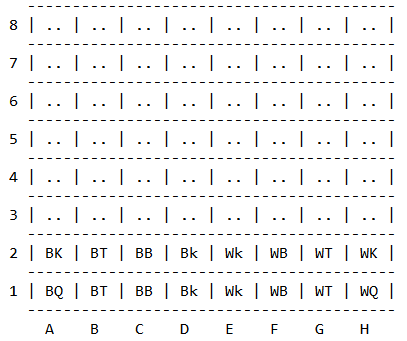
\includegraphics[scale = 0.4]{InitialBoard.png}
	\caption{Layout de jogo inicial.}
\end{figure}	

Uma representação interna possível do tabuleiro a meio do jogo como a acima apresentada  traduz-se no seguinte output de consola
no SICStus:
 \begin{figure}[H]
\centering
	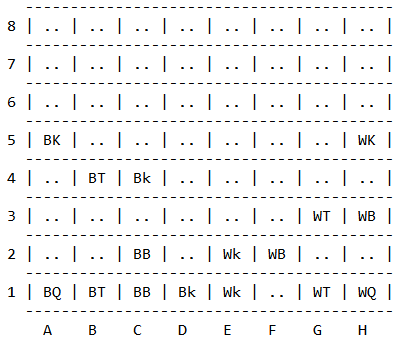
\includegraphics[scale = 0.4]{MidBoard.png}
	\caption{Layout de jogo a meio.}
\end{figure}	

Ainda, uma possível representação do tabuleiro num estado de jogo final será a seguinte: 
 \begin{figure}[H]
\centering
	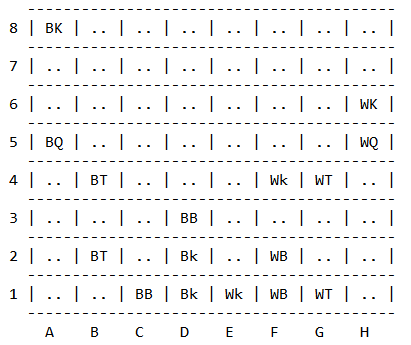
\includegraphics[scale = 0.4]{EndBoard.png}
	\caption{Layout de jogo final.}
\end{figure}	
\begin{center}
\begin{tabular}{c}
\begin{lstlisting}
/* Associates each number 
with a chess piece */
translate(0,T) :- T = '..'.
translate(1,T) :- T = 'WK'.
translate(2,T) :- T = 'WQ'.
translate(3,T) :- T = 'WT'.
translate(4,T) :- T = 'WB'.
translate(5,T) :- T = 'Wk'.
translate(6,T) :- T = 'BK'.
translate(7,T) :- T = 'BQ'.
translate(8,T) :- T = 'BT'.
translate(9,T) :- T = 'BB'.
translate(10,T) :- T = 'Bk'.

/* Recursive function to 
print current board state */
printBoard([],[]) :-
    write('  ------------------'), nl,
    write(' A B C D E F G H ').

printBoard([Line|Board],
	[LineNumb|Remainder]) :-
      write('  ----------------'),  nl,
      write(LineNumb), write(' '),
      printLine(Line),
      write('|'), nl,
      printBoard(Board,Remainder).


/* Recursive function to 
print each board's line */
printLine([]).
printLine([Head|Tail]) :-
      translate(Head,T),
      write('|'),
      write(T),
      printLine(Tail).

\end{lstlisting}
\end{tabular}
\end{center}
O tabuleiro inicial de jogo é criado usando o predicado initialBoard(X) em que X contem o tabuleiro inicial.

Para efeitos de apresentação foi construído o predicado printBoard(X) que recebe uma matriz X (lista de listas) e a imprime na consola.

É um predicado recursivo, que se auxilia noutro predicado, também ele recursivo, printLine(Y). que recebe uma matriz Y de elementos a imprimir na consola.

Assim, é passado ao predicado printBoard(X). o tabuleiro de jogo a immprimir. O mesmo separa a matriz na notação [H|T] em que 'H' representa a cabeça da lista (head) e 'T' a cauda da lista (tail). A cabeça apresenta-se como uma lista com os elementos da linha a imprimir, sendo passada ao printLine(X). . A cauda assume-se como uma lista de listas, sendo passada novamente (chamada recursiva) ao predicado printBoard(X). . Cada linha é processada recursivamente, dividida em [H|T], sendo que agora a cabeça da lista representa um elemento que é traduzido usando a chave referida e impresso na consola. A restante linha assume-se como uma lista de elementos a imprimir, sendo feita uma chamada recursiva a printLine(X). . Ambos os predicados apresentam como caso base o processamento de uma lista vazia.

Para efeitos de simplificação em termos de chamada na consola criou-se o predicado printBoard. de aridade 1
que efetua a chamada initialBoard(X), printBoard(X). .

%%%%%%%%%%%%%%%%%%%%%%%%%%
\section{Movimentos}

Cabeçalho do predicado de movimentação de uma peça:
\begin{lstlisting}
	movePiece(Row, Column, EndRow, EndColumn, Board)
\end{lstlisting}
Cabeçalho do predicado de captura de uma peça:
\begin{lstlisting}
	deletePiece(Row, Column, Board)
\end{lstlisting}
Para qualquer um destes predicados ser válido nenhuma das peças deve colocar o reio inimigo em cheque ou que o próprio rei em cheque:


\section{Bibliography}

%\bibliography{biblist}

[1] \href{https://lichess.org/variant/racingKings}{Lichess}

[2] \href{http://www.chessvariants.com/diffobjective.dir/racing.html}{Chess Variants}

[3] \href{https://en.wikipedia.org/wiki/V._R._Parton#Racing_Kings}{Wikipedia}

[4] \href{http://brainking.com/pt/GameRules?tp=125}{Brain King}

\end{document}
